\documentclass{article} % For LaTeX2e
\usepackage[final]{../colm2025_conference}

\usepackage{microtype}
\usepackage{hyperref}
\usepackage{url}
\usepackage{amsthm}
\usepackage{amsmath}
\usepackage{amssymb}
\usepackage{pifont}% http://ctan.org/pkg/pifont
\usepackage{booktabs}
\usepackage{soul}
\usepackage{cancel}
\usepackage{algorithm}
\usepackage{algpseudocode}
\usepackage{graphicx}
\usepackage{subfig}
\usepackage{tablefootnote}
\usepackage{multicol}
\theoremstyle{definition}
\newtheorem{theorem}{Theorem}[section]
% \newtheorem{proof}{Proof}[section]

\usepackage{lineno}
\newcommand{\cmark}{\ding{51}}%
\newcommand{\xmark}{\ding{55}}%

\definecolor{darkblue}{rgb}{0, 0, 0.5}
\hypersetup{colorlinks=true, citecolor=darkblue, linkcolor=darkblue, urlcolor=darkblue}


\title{Odyssey Final Report - RLVR For Reasoning LLMs}

\author{\textbf{BEH} Chuen Yang}

\newcommand{\fix}{\marginpar{FIX}}
\newcommand{\new}{\marginpar{NEW}}

\begin{document}

\ifcolmsubmission
\linenumbers
\fi

\maketitle
% - Congrats on finishing the LLM RL training and implementing your own task!
% - In the final two weeks, let’s explore a little bit more on LLM RL and wrap up this project in a report.
% (week 12, you can finish the coding and experiments without writing the report; you can put the results in the final report) 
% Continuing the GSM8k task, let’s consider another reward function. 
% Now we not only want the LLM output formatted and correct answer, we also want the answer to be as short / concise as possible. 
% Design the reward function, run the experiments, and compare with your old runs with analysis.

% - Lastly, write a final report for the WHOLE project. Make it short (<= 5 pages without references). 
% Make it comprehensive (include introduction, method, experiments, and conclusion;
% mirror a research paper that you read.).
%  A tip is that you can copy-paste from your previous report about the RL equations, LLM basics and so on, and summarize them in a concise way.
% Please include the experimental results of week 12 in the report.
% There’s no need to submit at the end of week 12; you can submit the code and final report at the end of week 13.

\begin{abstract}
    This final report summarizes the work done throughout the past weeks on Reinforcement Learning (RL), Large Language Models (LLMs),
    and RL with Verifiable Rewards (RLVR) in LLMs, culminating in a report detailing
    how RLVR can be used to train LLMs to perform reasoning tasks.
    This report presents most of the key results and findings from all weeks of the project, and it is hoped
    that the report serves as a good roadmap for understanding RLVR's potential to elicit reasoning capabilities in LLMs.
\end{abstract}

\section{Introduction}
Large Language Models (LLMs) have long been demonstrated capable of performing a staggering variety of tasks
in the Natural Language Processing (NLP) domain, ranging from text generation, 
sentiment analysis, to machine translation, question answering (\cite{Brown-et-al-2020}),
and in recent years, even complex reasoning tasks (\cite{tulu3, grpo, r1}).

By gaining deeper insights and practical experience in training LLMs with RLVR,
one can become better equipped to understand why LLMs are capable of reasoning,
how they fall short, and to what extent RLVR can be used to improve their reasoning capabilities.

\section{Background}

This section informally summarizes the key concepts for understanding
RLVR. More details can be found in the Appendices (where applicable)
as well as in previous weeks' works.

\subsection{LLMs}
As their name partly suggests, LLMs are a class of neural networks 
which attempt to learn the statistical distribution of natural language
(\cite{Zhao-et-al-2023, Karpathy-2025}). Especially in the modern context,
LLMs are \textbf{by and large} \footnote{Exceptions exist and are mentioned in \cite{wk5}. They are omitted here for brevity.} characterized by the following properties (\cite{wk5}):
\begin{itemize}
    \item LLMs model language \textit{causally} (\cite{Jurafsky-2024, Karpathy-2025}).
    \item LLMs adopt \textit{some variant of the Transformer architecture} (\cite{Vaswani-et-al-2017}).
    \item LLMs require a lot of data (often in the tens of terabytes (\cite{Karpathy-2025})) to train.
    \item LLMs typically have \textit{billions or even trillions} of parameters.
    \item Modern LLMs typically have \textit{diverse capabilities}, (\cite{Brown-et-al-2020})
        such as generating coherent text, following instructions, 
        and even engaging in conversations.
\end{itemize}

\subsubsection{How are LLMs trained?}
Per \cite{Karpathy-2025}, LLMs typically undergo multiple stages of training,
developing different capabilities at each stage.

Firstly, during \textit{pre-training}, LLMs are trained on a large corpus of text data
to learn general language patterns and structures by optimizing the objective in Equation \eqref{eq:pretrain-obj}.
This stage is typically \textit{self-supervised} in that the corpus
provides both the conditioning context and the target output, eliding
the need for human-curated labels. \footnote{
    See Appendix \ref{sec:cs-nanogpt} and (\cite{wk8})
    for an experiment on pre-training a small LLM on the TinyShakespeare corpus (\cite{tinyss, tinyss2}).
}
Next, some LLMs (\cite{InstructGPT-2022}) undergo \textit{supervised fine-tuning} on more specialized corpora to adapt 
their capabilities to specific tasks or domains (\cite{radford-et-al-2019,Brown-et-al-2020}).
While the objective is identical to Equation \eqref{eq:pretrain-obj} (\cite{wk5}),
the corpus \textit{consists of human-annotated examples} and 
the objective \textit{does not consider the log-likelihoods of the prompt tokens} (
    since strictly speaking, the prompt tokens are not part of the target output
).

Finally, most modern LLMs (\cite{tulu3, r1}) undergo \textit{reinforcement learning post-training},
such as RL with Human Feedback (RLHF) (\cite{Christiano-et-al-2017, InstructGPT-2022})
or RLVR (\cite{tulu3, grpo, r1}) to refine their output quality and alignment with human preferences.
We defer discussion of RLVR to Section \ref{sec:rlvr}, as it is the main focus of this report.

\subsection{RL}

In the general case, RL is a machine learning paradigm
where an agent learns to take a sequence of \textit{actions} 
in an \textit{environment} so as to to maximize cumulative reward (\cite{Sutton-and-Barto-1998}).

\subsubsection{RL Problems as Markov Decision Processes (MDPs)}
Most commonly, RL problems are formulated as MDPs
by \textit{assuming the Markov property}, where environment dynamics
only depend on the current state and action
(\cite{SpinningUp-2018, Levine-et-al-2023, Sutton-and-Barto-1998}) \footnote{
    A formal treatment of the following paragraph is given in Appendix \ref{sec:rl-obj}.
} This \textit{Markov assumption} is \textbf{key} to 
enabling the theoretical performance guarantees of many RL algorithms (\cite{Sutton-and-Barto-1998}).

Typically, an agent interacts with the environment via a \textit{parameterized, stochastic} policy
to collect experiences known as \textit{trajectories} or \textit{episodes}.
The agent then uses these trajectories to update its policy parameters
in a way that maximizes the expected cumulative reward
(\cite{Sutton-and-Barto-1998, SpinningUp-2018, Levine-et-al-2023}).

\subsubsection{Policy Gradient Methods}
Where RLVR is concerned, we are primarily interested in \textit{policy gradient methods} (\cite{wk2, SpinningUp-2018, Weng-2018}),
whose direct optimization on the RL objective in Equation \eqref{eq:rl-obj} is \textbf{uses the
observation that the expected cumulative reward is differentiable with respect to the policy parameters $\theta$} (\cite{SpinningUp-2018,Levine-et-al-2023,Weng-2018}).

This gives rise to a simple gradient ascent algorithm (\cite{wk2}) which a wide variety of algorithms like
REINFORCE (\cite{Williams-1992}),
Proximal Policy Optimization (PPO) (\cite{ppo}),
and Group Relative Policy Optimization (GRPO) (\cite{grpo}) are ultimately based on,
the details of which we relegate to Algorithm \ref{alg:reinforce} in Appendix \ref{sec:alg-reinforce}.

\subsubsection{Special Mention: GRPO}
A significant algorithm distinguished for its use in RLVR
is the Group Relative Policy Optimization (GRPO) algorithm (\cite{grpo}).\footnote{
    A summary of the GRPO Objective may be found in Appendix \ref{sec:grpo-obj}.
}
It is best described as a \textit{computationally-motivated variant} of PPO (\cite{ppo}) without 
a neural network baseline, which allows it to optimize LLMs on a tight memory budget, and has
been shown to be effective in training LLMs with RLVR (\cite{grpo, r1}).

\section{RLVR} \label{sec:rlvr}

At the intersection of RL and LLMs lies RLVR, which is characterized
by its use of RL to steer LLMs' outputs towards \textit{verifiably correct} ones,
according to task-specific criteria.
(\cite{tulu3, grpo, r1}).

This method is not only very simple to implement and able to extend
the frontier of LLM capabilities (\cite{tulu3, r1}), but it also 
escapes many of the usual pitfalls associated with RL on LLMs. For example, models trained on RLHF (\cite{InstructGPT-2022})
can provide \textit{incorrect, but convincing} answers to questions,
(\cite{Wen-et-al-2024}), or learn mismatched preferences due to biases mentioned in \cite{pitis-2023}.

Formally speaking, RLVR is typically formulated as a contextual bandit problem (\cite{Sutton-and-Barto-1998, contextualbandit})
(as with other RL methods on LLMs), where each model output $(o_1, \dots, o_n)$
denotes a \textit{single action}. A sample objective for RLVR may be obtained 
by considering Section \ref{sec:rlvr-obj}.

\section{Experiments}

Equipped with the requisite background knowledge on RLVR, we can now proceed
to explore how LLMs can be effectively trained to perform reasoning tasks with
this technique.

While this section is a partial summary of the work done in \cite{wk10},
it also contains new experiments and findings contributing to our knowledge
of reward function design in RLVR.

As in \cite{wk10}, we will be testing small, base language models
on the GSM8K dataset (\cite{gsm8k}) and evaluating their Pass@1 performance
on a small subset of holdouts. \textbf{However, we will also be varying the reward function
in order to \textit{also minimize} the length of models' responses, in addition
to maximizing the correctness of their answers.}

\subsection{GSM8K Dataset}

GSM8K (\cite{gsm8k}) is a grade school level math problem dataset consisting
of 8,792 word problems. All demand a single integer as the answer, and all
were deliberately designed to be solvable by elementary school students.

Due to the natural language format, this task is difficult to solve algorithmically.
Instead, it concurrently assesses models' ability to parse diverse problem statements, 
reason about numbers, and perform arithmetic operations accurately (\cite{gsm8k}).

\subsection{Experimental Configurations}

For all experiments, we relied on an adapted version of the nano-aha-moment repository (\cite{nano-aha-moment}),
which provides a faithful single-file implementation of the GRPO algorithm (\cite{grpo})
and a simple training pipeline for arbitrary LLMs on arbitrary datasets (as long
as they are supported by HuggingFace Transformers (\cite{hf-transformers})) (\cite{wk10}).

Training was alternately conducted on a single NVIDIA 4090 GPU with 48GB of VRAM,
and a single NVIDIA 3090 GPU with 24GB of VRAM \footnote{
    Thanks Chann.
}. All runs took a combined $\sim$ 40 hours of wall-clock time to complete.
As in \cite{wk10}, we only performed one trial for each reward function 
due to compute restrictions.

\subsection{Reward Modelling}

Owing to its central role as an independent variable in our experiment,
we go into further detail on the design of the reward function in \cite{wk10}.

In \cite{wk10}, our reward function is a variant of \cite{nano-aha-moment}'s, 
and it is a more permissive variant of that
described by \cite{r1}:
\begin{equation} \label{eq:control-reward-fn}
    \begin{array}{rl}
        R(s, a) &= C(s, a) + F(s, a) \\
        & =\begin{cases}
            1 & \text{if } a \text{ contains the correct answer} \\
            0 & \text{otherwise}
        \end{cases} \\
        & + \begin{cases}
            1 & \text{if } a \text{ contains thinking, $\backslash n$, and a single integer answer.} \\
            0.5 & \text{if } a \text{ contains thinking, $\backslash n$, and any answer.} \\
            0 & \text{otherwise}
        \end{cases}
    \end{array}
\end{equation}

We speculate the additional half-reward clause encourages the model to produce
valid answers even if they do not obey the strict response format (\cite{wk10}).

\subsection{Hyperparameters}

The numerical hyperparameters used in our experiments were identical to those used in \cite{wk10}.
For more details, please refer to Table \ref{tab:universal-hyperparams}.

In attempting to minimize the length of the model's responses,
we also considered the following reward functions (the default reward function from \cite{wk10} 
is also included for comparison):
\begin{table}[h]
    \centering
    \begin{tabular}{|p{0.2\textwidth}|p{0.6\textwidth}|p{0.3\textwidth}|}
        \hline
        \textbf{Reward Function} & \textbf{Description} & \textbf{Function Name} \\
        \hline
        Control (\cite{wk10}) 
        & $r(s, a) = R(s, a)$ (Equation \ref{eq:control-reward-fn})
        & \texttt{noop\_decay}
        \\ \hline
        Linear Penalty 
        & $$r(s, a) = \left(1 - 0.5 clip\left(\frac{len(a)}{L}, 1\right)\right) R(s, a)$$
        & \texttt{linear\_length\_decay}
        \\ \hline 
        Quadratic Penalty
        & $$r(s, a) = \left(1 - 0.5 clip\left(\left(\frac{len(a)}{L}\right)^2, 1\right)\right) R(s, a)$$ 
        & \texttt{quadratic\_length\_decay}
        \\ \hline
        Batch Exponential Moving Average Penalty
        & $$r(s, a) = \beta R(s, a)$$ 
        \newline
        $\beta = \begin{cases}
            1.2 & \text{if } a < \texttt{avg\_response\_length} - 10 \\
            0.8 & \text{if } a > \texttt{avg\_response\_length} + 10 \\
            1.0 & \text{otherwise}
        \end{cases}$
        & \texttt{batch\_exp\_avg\_decay}
        \\ \hline
        ShorterBetter (\cite{ShorterBetter})
        & $$r(s, a) = R(s, a) - 0.0005 |len(a) - l_{SOL}|$$
        \newline
        $l_{SOL} = \begin{cases}
            min(len(a_1), \dots, len(a_n)) & \text{if any } a_i \text{ is correct} \\
            \frac{1}{n}\sum_{i = 1}^{n} len(a_i) & \text{otherwise}
        \end{cases}$
        & None (See \texttt{nano\_r1\_gsm8k} \newline \texttt{\_shorterbetter.py})
        \\ \hline
    \end{tabular}
    \caption{Reward Functions used in our experiments.}
    \label{tab:reward-functions}
\end{table}
\section{Results}
\subsection{Pass@1 Performance}


\section{Discussion}

\bibliographystyle{../colm2025_conference}
\bibliography{wk12}
\appendix
\section{Objective Functions}
\subsection{LLM Pre-training Objective}

Where $\theta^{*}$ are the model parameters and $N$ is the model's context length, 
an optimal language model $LM_{(\theta^{*}, N)}$
maximizes the likelihood of the next token given all previous tokens, across all training examples
$\left\{\{x_{j + i}\}_{i = 0}^{N - 1}\right\}_{j = 1}^{M - N}$ 
in a corpus of size $M$:
\begin{equation} \label{eq:pretrain-obj}
    \theta^{*} = \underset{\theta}{\arg\min} \sum_{j = 1}^{M - N} \left[\sum_{i = 0}^{N - 1} -\log P_{\theta}(x_{j + i} | x_j, \cdots, x_{< (j + i)})\right]
\end{equation}

\subsection{General RL Objective}
\label{sec:rl-obj}

Formally speaking, an MDP is defined as a tuple $(\mathcal{S}, \mathcal{A}, \tau, r, \gamma)$, 
where $\mathcal{S}$ is the set of \textit{states} in the environment, 
$\mathcal{A}$ is the set of \textit{actions} the agent can take,
$\tau: \mathcal{S} \times \mathcal{A} \times \mathcal{S} \rightarrow [0, 1]$ is the \textit{transition function},
$r: \mathcal{S} \times \mathcal{A} \times \mathcal{S} \rightarrow \mathbb{R}$ is the \textit{reward function}, and 
$\gamma \in [0, 1]$ is (an optional) \textit{discount factor}.


Typically, an agent interacts with the environment 
via a \textit{parameterized, stochastic} policy $\pi_\theta: \mathcal{S} \times \mathcal{A} \rightarrow [0, 1]$,
in an \textit{episodic} manner, where $s_0 \sim \rho_0$ (the initial state distribution),
and $\forall_{0 \leq k < n}\left(a_{k} \sim \pi_\theta(s_k), s_{k+1} \sim \tau(s_k, a_{k})\right)$ (\cite{wk1}). 
The agent thus induces a sequence of interactions $T = (s_0, a_0, s_1, a_1, \ldots, s_n)$
(a \textit{trajectory}), which should be regarded analogously to one
of many games of Tic-Tac-Toe, or a single playthrough of a video game.

Simply put, the optimal policy $\pi_{\theta^{*}}$ is the one that maximizes the \textit{expected cumulative reward} (\cite{wk2}):
\begin{equation} \label{eq:rl-obj}
    \pi_{\theta^{*}} = {\displaystyle \arg\max_{\pi_\theta} \underset{T \sim \pi_{\theta}}{\mathbb{E}} \left[ \sum_{t=0}^{n} \gamma^t r(s_t, a_t) \right] }
\end{equation}

\subsection{GRPO Objective}
\label{sec:grpo-obj}

Consider a policy network $\pi_\theta$ and critic network $V_\phi$ in a single-state,
single-action armed bandit environment (\cite{Sutton-and-Barto-1998, contextualbandit}) 
with state $s$ and action $a = (o_1, \dots, o_n)$,
where $o_k$ is the $k$-th output token of the language model.
Then the GRPO objective is defined as follows (\cite{grpo, wk10}):
\begin{equation}
    \label{eq:grpo-obj}
    \begin{array}{rl}
        \mathcal{J}(\theta) &= \mathbb{E}_{(s, o_1, \dots, o_n) \sim \pi_\theta} \left[ 
            \displaystyle
            \frac{1}{n} \sum_{k = 1}^n \min \left\{
                \frac{\pi_\theta(o_k|s, o_{< k})}{\pi_{\theta_{old}}(o_k|s, o_{< k})} A(s, a),
                g(s, a)
            \right\}
        \right] {\displaystyle - \lambda D_{KL}(\pi_\theta || \pi_{\theta_{old}})} \\
    \end{array}
\end{equation}
where ${\displaystyle g(s, a) = clip\left(\frac{\pi_\theta(o_k|s, o_{< k})}{\pi_{\theta_{old}}(o_k|s, o_{< k})}, 1 - \epsilon, 1 + \epsilon \right) A(s, a)}$,
and $\pi_{\theta_{old}}$ is the policy network from the previous GRPO step.

\subsection{RLVR Objective}
\label{sec:rlvr-obj}

GRPO (\cite{grpo}) has historically been the algorithm of choice for RLVR (\cite{r1, grpo}),
hence an objective function for RLVR can simply be \ref{eq:grpo-obj}.

\section{Miscellaneous Case Studies}

\subsubsection{Case Study: REINFORCE} \label{sec:cs-reinforce}
In \cite{wk3}, we experimented with a simple RL training pipeline by 
\cite{Levine-et-al-2023} to train a simple network on the CartPole environment (\cite{Towers-et-al-2024}).
 
\subsection{Case Study: nanoGPT} \label{sec:cs-nanogpt}
In \cite{wk8}, experiments in pre-training a small LLM on the TinyShakespeare corpus (\cite{tinyss, tinyss2}) were
conducted with nanoGPT (\cite{nanoGPT}). While the details of the experiment can be found in \cite{wk8},
we summarize the key findings here:
\begin{figure}
    \centering
    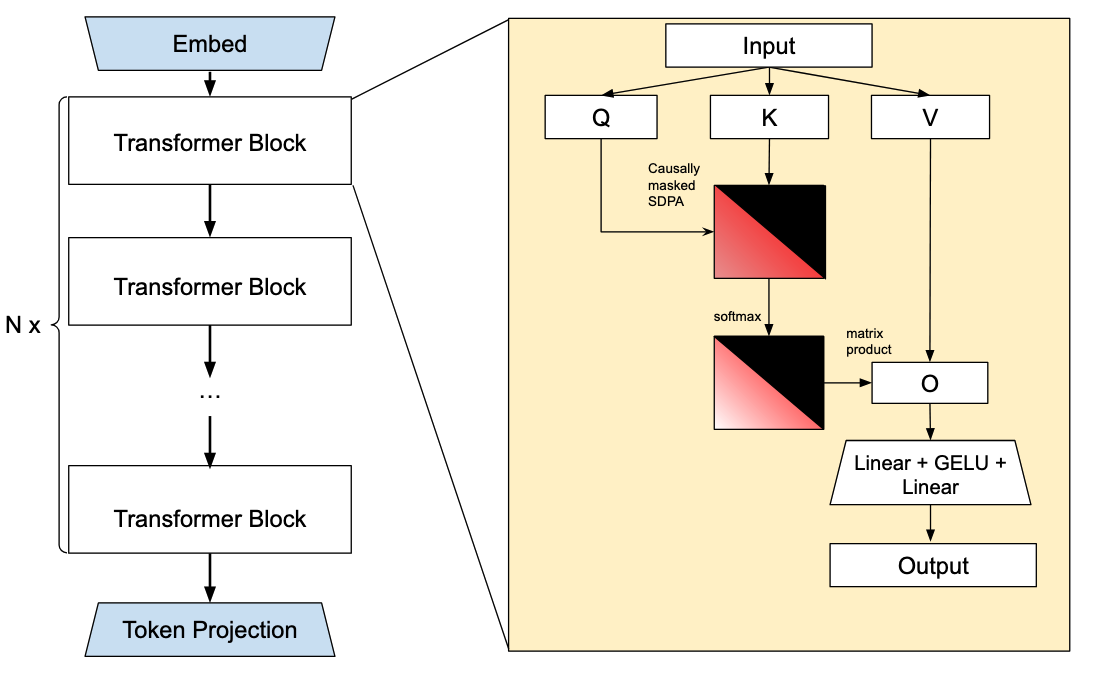
\includegraphics[width=0.45\textwidth, height=0.15\textheight]{images/gpt_arch.png}
    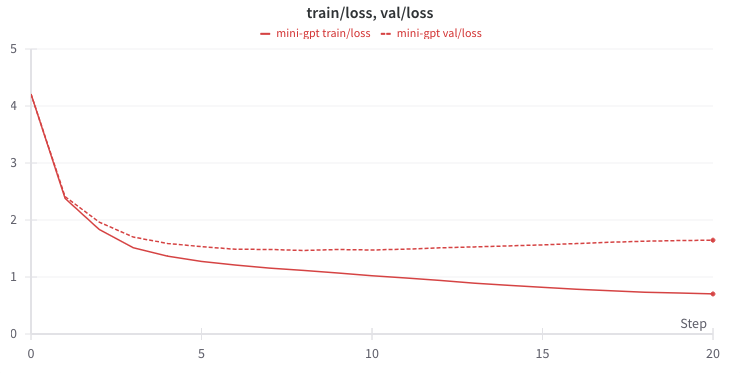
\includegraphics[width=0.45\textwidth, height=0.15\textheight]{images/loss_curves.png}
    \caption{(Left) The architecture of nanoGPT, illustrated. (Right) The training loss curves of the pre-trained nanoGPT model.}
    \label{fig:nanoGPT-sample}
\end{figure}
\begin{itemize}
    \item Despite being tokenized on a character level, the model could generate valid whole words
         with few to no errors.
    \item The model could generate text that (superficially) resembled the training corpus.
    \item The model often produced nonsensical text.
\end{itemize}


\section{Policy Gradient Algorithm}
\label{sec:alg-reinforce}

\begin{algorithm}[H] 
    \caption{Improved Policy Gradient Algorithm}
    \label{alg:reinforce}
    \begin{algorithmic}[1]
        \State Input: Policy $\pi_\theta$, learning rate $\alpha$, baseline of choice $b(s_t)$
        \State Output: Updated policy $\pi_\theta$
        \While{not converged}
            \State Sample a batch of trajectories $T$ from the policy $\pi_\theta$
            \For{each trajectory $T$ in the batch}
                \State Compute the rewards-to-go $R_t$ for each time step $t$ in the trajectory
                \State Compute the baseline $b(s_t)$ for each time step $t$ in the trajectory
                \State Estimate $\nabla_\theta J(\pi_\theta) \approx \frac{1}{m} \left(\sum_{t = 0}^{n} R_t - b(s_t)\right) \left( \sum_{t=0}^{n} \nabla_\theta \log(\pi_\theta(a_t | s_t)) \right)$
            \EndFor
            \State $\theta \leftarrow \theta + \alpha \nabla_\theta J(\pi_\theta)$
        \EndWhile
    \end{algorithmic}
\end{algorithm}

\section{Numerical Hyperparameters}

As in \cite{wk10}, we used the following hyperparameters for all runs of the GSM8K task:
\begin{table}[h]
    \centering
    \begin{tabular}{|l|c|}
        \hline
        \textbf{Hyperparameter} & \textbf{GSM8K} \\
        \hline
        Model Family & Qwen2.5 (\cite{Qwen-et-al-2025}) \\
        \hline
        Model Scale & 1.5B \\
        \hline
        Batch Size & 16 \\
        \hline
        Learning Rate & 1e-6 \\
        \hline
        Max. Response Length ($L$) & 512 \\
        \hline
        Completions per Task & 8 \\
        \hline
        Episodes per GRPO Iteration & 16\\
        \hline
        KL Divergence Coefficient $\lambda$ & 0 \\
        \hline
        Random Seed & 42 \\
        \hline
    \end{tabular}
    \caption{Universal Hyperparameters across our experiments.}
    \label{tab:universal-hyperparams}
\end{table}

\end{document}